% =========================================================================
% capitulos/03_actividades_realizadas.tex
% Capítulo III: Actividades Realizadas
% =========================================================================

\section{Actividades Realizadas}

En este capítulo se detalla el núcleo técnico del informe de prácticas preprofesionales, abarcando desde el diagnóstico de la situación previa hasta el desarrollo y validación de las actividades asignadas.

\subsection{Situación actual (previa al desarrollo)}
Describa el estado inicial de los procesos, sistemas o infraestructura en la institución receptora antes de la ejecución de las prácticas. Es importante destacar las limitaciones tecnológicas o cuellos de botella existentes que motivaron la asignación del proyecto.

\subsection{Problemática}
Sintetice de forma puntual los problemas centrales identificados:
\begin{enumerate}
  \item \textbf{Incompatibilidad y dispersión de datos:} Existencia de silos de información aislados que dificultan la consolidación de reportes.
  \item \textbf{Procesos operativos manuales:} Dependencia excesiva de registros manuales susceptibles a errores humanos y retrasos operativos.
  \item \textbf{Falta de escalabilidad tecnológica:} Infraestructura de software rígida o heredada con elevado costo de mantenimiento y escasa capacidad de integración.
\end{enumerate}

\subsection{Objetivos}

\subsubsection{General}
Formule un objetivo general en verbo infinitivo que sintetice la meta primordial del proyecto (por ejemplo: \textit{Diseñar e implementar un sistema de información web para la gestión operativa y control de procesos en la empresa receptora}).

\subsubsection{Específicos}
Plantee de 3 a 5 objetivos específicos ordenados lógica y cronológicamente:
\begin{itemize}
  \item Realizar el levantamiento de requerimientos y el análisis de la arquitectura técnica del sistema.
  \item Diseñar el modelo de datos relacional y las interfaces gráficas de usuario siguiendo criterios de usabilidad.
  \item Desarrollar los módulos centrales de procesamiento lógico y servicios web bajo una arquitectura modular.
  \item Ejecutar pruebas de integración y validación funcional para verificar el correcto comportamiento de la solución.
\end{itemize}

\subsection{Alcance}
Delimite con precisión las fronteras del proyecto: qué módulos, funcionalidades y plataformas quedan comprendidas, así como aquellas características que quedan explícitamente fuera del ámbito de ejecución.

\subsection{Justificación}
Fundamente la importancia de la intervención técnica, explicando los beneficios operativos, económicos, tecnológicos y de gestión que la organización obtiene tras la culminación exitosa de las actividades.

\subsection{Equipo de Trabajo}
Describa la composición del equipo con el cual se coordinaron las labores:
\begin{itemize}
  \item \textbf{Responsable del Área / Product Owner:} Encargado de validar prioridades del negocio.
  \item \textbf{Líder Técnico / Supervisor:} Encargado de la supervisión y soporte técnico directo.
  \item \textbf{Practicante Preprofesional:} Responsable del diseño, codificación y pruebas del sistema.
\end{itemize}

\subsection{Cronograma de Actividades}
En la \autoref{tab:cronograma_actividades} se expone la distribución temporal planificada para las fases del proyecto a lo largo del periodo de prácticas.

\begin{table}[htbp]
  \centering
  \caption{Cronograma de ejecución de actividades por semanas.}
  \label{tab:cronograma_actividades}
  \begin{tabularx}{0.95\textwidth}{Xcccc}
    \toprule
    \textbf{Fase / Actividad} & \textbf{Mes 1} & \textbf{Mes 2} & \textbf{Mes 3} & \textbf{Entregable} \\
    \midrule
    1. Análisis de Requerimientos & \textbf{X} & & & Documento ERS \\
    2. Diseño de Arquitectura y Base de Datos & \textbf{X} & \textbf{X} & & Modelo ER / Mockups \\
    3. Construcción de Módulos Core & & \textbf{X} & \textbf{X} & Código Fuente v1.0 \\
    4. Pruebas y Despliegue en Pruebas & & & \textbf{X} & Reporte de QA \\
    5. Documentación y Manuales de Usuario & & & \textbf{X} & Manual Técnico \\
    \bottomrule
  \end{tabularx}
  \fuente{Elaboración propia.}
\end{table}

\subsection{Desarrollo de las Actividades}

En esta sección se detalla la implementación técnica, arquitectura adoptada y resultados obtenidos en cada etapa.

\subsubsection{Ejemplo de Inclusión de Diagramas y Figuras}
En la \autoref{fig:arquitectura_muestra} se esquematiza un diagrama representativo del diseño modular de componentes.

\begin{figure}[htbp]
  \centering
  \IfFileExists{assets/figuras/ejemplo_figura.png}{%
    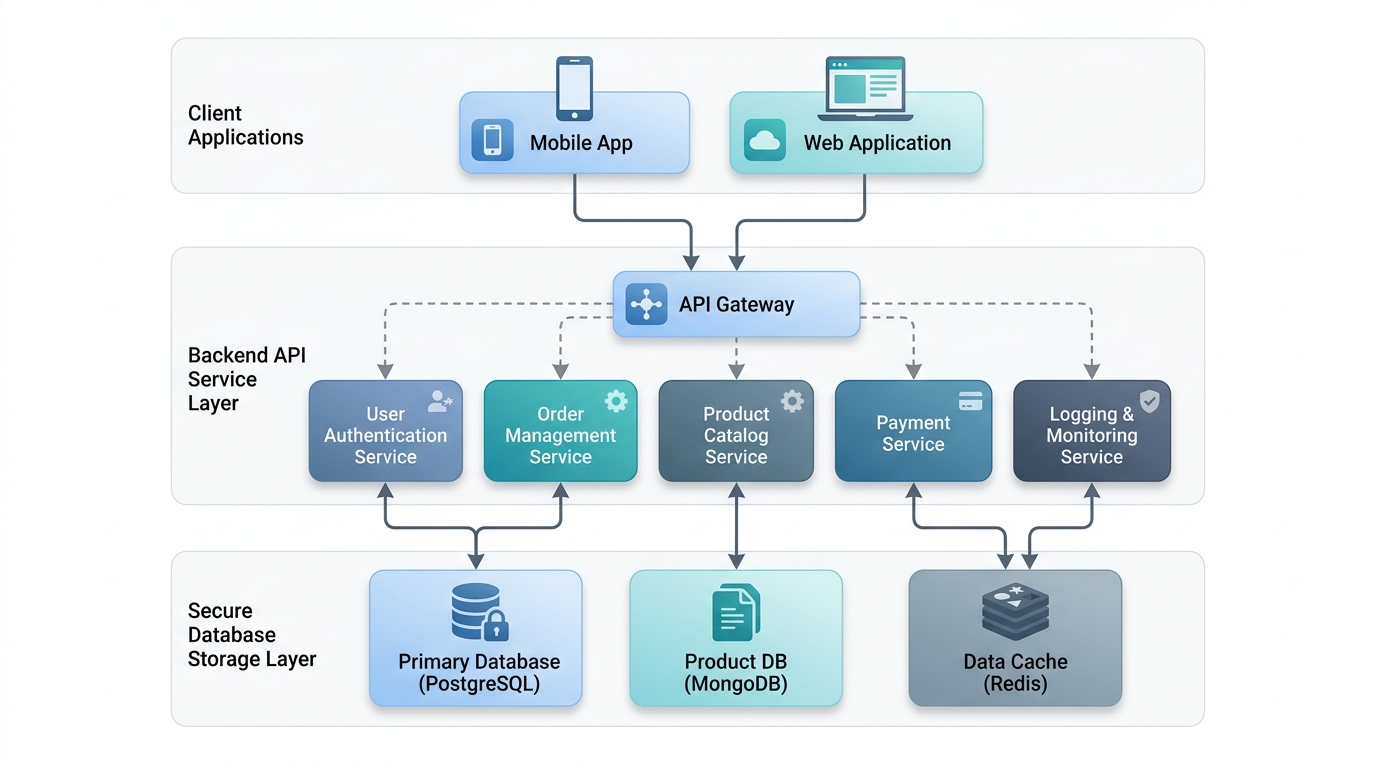
\includegraphics[width=0.75\textwidth]{assets/figuras/ejemplo_figura.png}%
  }{%
    \fbox{\parbox{0.7\textwidth}{\centering\vspace{2cm} [Coloque su figura en assets/figuras/] \vspace{2cm}}}%
  }
  \caption{Esquema conceptual de la arquitectura modular implementada.}
  \label{fig:arquitectura_muestra}
  \fuente{Elaboración propia.}
\end{figure}

\subsubsection{Ejemplo de Bloques de Código Fuente}
Para documentar algoritmos, controladores o esquemas de configuración, utilice el entorno estándar \texttt{lstlisting}:

\begin{lstlisting}[language=Python, caption={Controlador de ejemplo para el procesamiento de solicitudes.}, label={lst:ejemplo_codigo}]
# Controlador modular de ejemplo
class GestionProcesos:
    def __init__(self, repositorio_datos):
        self.repositorio = repositorio_datos

    def registrar_actividad(self, actividad_id: str, detalle: dict) -> bool:
        """Valida y registra una nueva actividad en el repositorio."""
        if not actividad_id or not detalle:
            raise ValueError("Parámetros de actividad inválidos.")
        return self.repositorio.guardar(actividad_id, detalle)
\end{lstlisting}
